% ******************************* PhD Thesis Template **************************
% Please have a look at the README.md file for info on how to use the template

\documentclass[a4paper,12pt,times,numbered,print,index]{Classes/PhDThesisPSnPDF}

% ******************************************************************************
% ******************************* Class Options ********************************
% *********************** See README for more details **************************
% ******************************************************************************

% `a4paper'(The University of Cambridge PhD thesis guidelines recommends a page
% size a4 - default option) or `a5paper': A5 Paper size is also allowed as per
% the Cambridge University Engineering Deparment guidelines for PhD thesis
%
% `11pt' or `12pt'(default): Font Size 10pt is NOT recommended by the University
% guidelines
%
% `oneside' or `twoside'(default): Printing double side (twoside) or single
% side.
%
% `print': Use `print' for print version with appropriate margins and page
% layout. Leaving the options field blank will activate Online version.
%
% `index': For index at the end of the thesis
%
% `draftclassic': For draft mode without loading any images (same as draft in book)
%
% `draft': Special draft mode with line numbers, images, and water mark with
% timestamp and custom text. Position of the text can also be modified.
%
% `abstract': To generate only the title page and abstract page with
% dissertation title and name, to submit to the Student Registry
%
% `chapter`: This option enables only the specified chapter and it's references
%  Useful for review and corrections.
%
% ************************* Custom Page Margins ********************************
%
% `custommargin`: Use `custommargin' in options to activate custom page margins,
% which can be defined in the preamble.tex. Custom margin will override
% print/online margin setup.
%
% *********************** Choosing the Fonts in Class Options ******************
%
% `times' : Times font with math support. (The Cambridge University guidelines
% recommend using times)
%
% `fourier': Utopia Font with Fourier Math font (Font has to be installed)
%            It's a free font.
%
% `customfont': Use `customfont' option in the document class and load the
% package in the preamble.tex
%
% default or leave empty: `Latin Modern' font will be loaded.
%
% ********************** Choosing the Bibliography style ***********************
%
% `authoryear': For author-year citation eg., Krishna (2013)
%
% `numbered': (Default Option) For numbered and sorted citation e.g., [1,5,2]
%
% `custombib': Define your own bibliography style in the `preamble.tex' file.
%              `\RequirePackage[square, sort, numbers, authoryear]{natbib}'.
%              This can be also used to load biblatex instead of natbib
%              (See Preamble)
%
% **************************** Choosing the Page Style *************************
%
% `default (leave empty)': For Page Numbers in Header (Left Even, Right Odd) and
% Chapter Name in Header (Right Even) and Section Name (Left Odd). Blank Footer.
%
% `PageStyleI': Chapter Name next & Page Number on Even Side (Left Even).
% Section Name & Page Number in Header on Odd Side (Right Odd). Footer is empty.
%
% `PageStyleII': Chapter Name on Even Side (Left Even) in Header. Section Number
% and Section Name in Header on Odd Side (Right Odd). Page numbering in footer


% ********************************** Preamble **********************************
% Preamble: Contains packages and user-defined commands and settings
% ******************************************************************************
% ****************************** Custom Margin *********************************

% Add `custommargin' in the document class options to use this section
% Set {innerside margin / outerside margin / topmargin / bottom margin}  and
% other page dimensions
\ifsetCustomMargin
  \RequirePackage[left=37mm,right=30mm,top=35mm,bottom=30mm]{geometry}
  \setFancyHdr % To apply fancy header after geometry package is loaded
\fi

% *****************************************************************************
% ******************* Fonts (like different typewriter fonts etc.)*************

% Add `customfont' in the document class option to use this section

\ifsetCustomFont
  % Set your custom font here and use `customfont' in options. Leave empty to
  % load computer modern font (default LaTeX font).
  %\RequirePackage{helvet}

  % For use with XeLaTeX
  %  \setmainfont[
  %    Path              = ./libertine/opentype/,
  %    Extension         = .otf,
  %    UprightFont = LinLibertine_R,
  %    BoldFont = LinLibertine_RZ, % Linux Libertine O Regular Semibold
  %    ItalicFont = LinLibertine_RI,
  %    BoldItalicFont = LinLibertine_RZI, % Linux Libertine O Regular Semibold Italic
  %  ]
  %  {libertine}
  %  % load font from system font
  %  \newfontfamily\libertinesystemfont{Linux Libertine O}
\fi

% *****************************************************************************
% **************************** Custom Packages ********************************

% ************************* Algorithms and Pseudocode **************************

%\usepackage{algpseudocode}


% ********************Captions and Hyperreferencing / URL **********************

% Captions: This makes captions of figures use a boldfaced small font.
%\RequirePackage[small,bf]{caption}

\RequirePackage[labelsep=space,tableposition=top]{caption}
\renewcommand{\figurename}{Fig.} %to support older versions of captions.sty


% *************************** Graphics and figures *****************************

%\usepackage{rotating}
%\usepackage{wrapfig}

% Uncomment the following two lines to force Latex to place the figure.
% Use [H] when including graphics. Note 'H' instead of 'h'
%\usepackage{float}
%\restylefloat{figure}

% Subcaption package is also available in the sty folder you can use that by
% uncommenting the following line
% This is for people stuck with older versions of texlive
%\usepackage{sty/caption/subcaption}
\usepackage{subcaption}

% ********************************** Tables ************************************
\usepackage{booktabs} % For professional looking tables
\usepackage{multirow}

%\usepackage{multicol}
%\usepackage{longtable}
%\usepackage{tabularx}


% *********************************** SI Units *********************************
\usepackage{siunitx} % use this package module for SI units


% ******************************* Line Spacing *********************************

% Choose linespacing as appropriate. Default is one-half line spacing as per the
% University guidelines

% \doublespacing
% \onehalfspacing
% \singlespacing


% ************************ Formatting / Footnote *******************************

% Don't break enumeration (etc.) across pages in an ugly manner (default 10000)
%\clubpenalty=500
%\widowpenalty=500

%\usepackage[perpage]{footmisc} %Range of footnote options


% *****************************************************************************
% *************************** Bibliography  and References ********************

%\usepackage{cleveref} %Referencing without need to explicitly state fig /table

% Add `custombib' in the document class option to use this section
\ifuseCustomBib
   \RequirePackage[square, sort, numbers, authoryear]{natbib} % CustomBib

% If you would like to use biblatex for your reference management, as opposed to the default `natbibpackage` pass the option `custombib` in the document class. Comment out the previous line to make sure you don't load the natbib package. Uncomment the following lines and specify the location of references.bib file

%\RequirePackage[backend=biber, style=numeric-comp, citestyle=numeric, sorting=nty, natbib=true]{biblatex}
%\bibliography{References/references} %Location of references.bib only for biblatex

\fi

% changes the default name `Bibliography` -> `References'
\renewcommand{\bibname}{References}


% ******************************** Roman Pages *********************************
% The romanpages environment set the page numbering to lowercase roman one
% for the contents and figures lists. It also resets
% page-numbering for the remainder of the dissertation (arabic, starting at 1).

\newenvironment{romanpages}{
  \setcounter{page}{1}
  \renewcommand{\thepage}{\roman{page}}}
{\newpage\renewcommand{\thepage}{\arabic{page}}}


% ******************************************************************************
% ************************* User Defined Commands ******************************
% ******************************************************************************

% *********** To change the name of Table of Contents / LOF and LOT ************

%\renewcommand{\contentsname}{My Table of Contents}
%\renewcommand{\listfigurename}{My List of Figures}
%\renewcommand{\listtablename}{My List of Tables}


% ********************** TOC depth and numbering depth *************************

\setcounter{secnumdepth}{2}
\setcounter{tocdepth}{2}


% ******************************* Nomenclature *********************************

% To change the name of the Nomenclature section, uncomment the following line

%\renewcommand{\nomname}{Symbols}


% ********************************* Appendix ***********************************

% The default value of both \appendixtocname and \appendixpagename is `Appendices'. These names can all be changed via:

%\renewcommand{\appendixtocname}{List of appendices}
%\renewcommand{\appendixname}{Appndx}

% *********************** Configure Draft Mode **********************************

% Uncomment to disable figures in `draftmode'
%\setkeys{Gin}{draft=true}  % set draft to false to enable figures in `draft'

% These options are active only during the draft mode
% Default text is "Draft"
%\SetDraftText{DRAFT}

% Default Watermark location is top. Location (top/bottom)
%\SetDraftWMPosition{bottom}

% Draft Version - default is v1.0
%\SetDraftVersion{v1.1}

% Draft Text grayscale value (should be between 0-black and 1-white)
% Default value is 0.75
%\SetDraftGrayScale{0.8}


% ******************************** Todo Notes **********************************
%% Uncomment the following lines to have todonotes.

%\ifsetDraft
%	\usepackage[colorinlistoftodos]{todonotes}
%	\newcommand{\mynote}[1]{\todo[author=kks32,size=\small,inline,color=green!40]{#1}}
%\else
%	\newcommand{\mynote}[1]{}
%	\newcommand{\listoftodos}{}
%\fi

% Example todo: \mynote{Hey! I have a note}

% ************************ Thesis Information & Meta-data **********************
% Thesis title and author information, refernce file for biblatex
% ************************ Thesis Information & Meta-data **********************
%% The title of the thesis
\title{Deep Neural Networks for Sound Type Classification}
%\texorpdfstring is used for PDF metadata. Usage:
%\texorpdfstring{LaTeX_Version}{PDF Version (non-latex)} eg.,
%\texorpdfstring{$sigma$}{sigma}

%% Subtitle (Optional)
%\subtitle{}

%% The full name of the author
\author{Xiaowei Jiang}

%% Department (eg. Department of Engineering, Maths, Physics)
\dept{Faculty IV: Electrical Engineering and Computer Science}

%% University and Crest
\university{Technology University of Berlin}
% Crest minimum should be 30mm.
\crest{
\includegraphics[width=0.2\textwidth]{./Figs/TU_Logo_kurz_RGB_rot}}
%% Use this crest, if you are using the college crest
%% Crest long miminum should be 65mm
%\crest{\includegraphics[width=0.45\textwidth]{University_Crest_Long}}

%% College shield [optional] 
% Crest minimum should be 30mm.
%\collegeshield{\includegraphics[width=0.2\textwidth]{CollegeShields/Kings}}

%% You can redefine the submission text:
% Default as per the University guidelines:
% ``This dissertation is submitted for the degree of''
%\renewcommand{\submissiontext}{change the default text here if needed}

%% Full title of the Degree
\degreetitle{Bachelor of Computer Science}

%% College affiliation (optional)
%\college{King's College}

%% Submission date
% Default is set as {\monthname[\the\month]\space\the\year}
\degreedate{September 2016} 

%% Meta information
\subject{LaTeX} \keywords{{LaTeX} {Bachelor Thesis} {Computer Science} {Technology University of
Berlin}}

% ***************************** Abstract Separate ******************************
% To printout only the titlepage and the abstract with the PhD title and the
% author name for submission to the Student Registry, use the `abstract' option in
% the document class.

\ifdefineAbstract
 \pagestyle{empty}
 \includeonly{Declaration/declaration, Abstract/abstract}
\fi

% ***************************** Chapter Mode ***********************************
% The chapter mode allows user to only print particular chapters with references
% Title, Contents, Frontmatter are disabled by default
% Useful option to review a particular chapter or to send it to supervisior.
% To use choose `chapter' option in the document class

\ifdefineChapter
 \includeonly{Chapter3/chapter3}
\fi

% ******************************** Front Matter ********************************
\begin{document}

\frontmatter

\begin{titlepage}
  \maketitle
\end{titlepage}


%% ******************************* Thesis Dedidcation ********************************

\begin{dedication} 

I would like to dedicate this thesis to my loving parents \dots

\end{dedication}
%% ******************************* Thesis Declaration ***************************

\begin{declaration}

I hereby declare that except where specific reference is made to the work of 
others, the contents of this dissertation are original and have not been 
submitted in whole or in part for consideration for any other degree or 
qualification in this, or any other university. This dissertation is my own 
work and contains nothing which is the outcome of work done in collaboration 
with others, except as specified in the text and Acknowledgements. This 
dissertation contains fewer than 65,000 words including appendices, 
bibliography, footnotes, tables and equations and has fewer than 150 figures.

% Author and date will be inserted automatically from thesis.tex \author \degreedate

\end{declaration}
%% ************************** Thesis Acknowledgements **************************

\begin{acknowledgements}      


And I would like to acknowledge ...


\end{acknowledgements}

% ************************** Thesis Abstract *****************************
% Use `abstract' as an option in the document class to print only the titlepage and the abstract.
\begin{abstract}
This is where you write your abstract ...
\end{abstract}


% *********************** Adding TOC and List of Figures ***********************

\tableofcontents

\listoffigures

\listoftables

% \printnomenclature[space] space can be set as 2em between symbol and description
%\printnomenclature[3em]

\printnomenclature

% ******************************** Main Matter *********************************
\mainmatter

\chapter{Background and Motivation}
\label{chap:backgrd}
%explain structure of this thesis
Nowadays neural networks and deep learning has become a hot topic in pattern recognition, speaker identification, image processing and many other fields. In this thesis, deep neural networks are used as a solution for sound type classification problem.
In Chapter \ref{chap:backgrd} some basic concepts related to sound type classification and neural networks are introduced. This thesis is based on part of works of the Two!Ears system. Sound type classification is a module of the Two!Ears system. These basic concepts are introduced in section \ref{sec:soundtc}. Section \ref{sec:deepNN} explains what DNNs are and introduces the Caffe framework, which is used for producing the experiment results in this thesis. After that, the main part of the thesis starts by exploring the architecture of neural networks applied to sound type classification. Three types of architectures are discussed in Chapter \ref{chap:architecture}. A good architecture doesn't solve the problem completely, overfitting is always a problem one should consider in machine learning problems. In Chapter \ref{chap:dataAug}, data augmentation is introduced to deal with the overfitting problem. Tuning parameters of deep neural networks requires a broad and lengthy exploration of the parameter space.  At last, a conclusion is drawn in Chapter \ref{chap:conclusion}. I will also talk about future works related to this topic.

\section{Sound Type Classification}
\label{sec:soundtc}
%goal:usually features are handcrafted by domain experts
In this thesis, sound type classification is a supervised machine learning problem, which serves as a module of the Two!Ears System. The training data set is the NIGENS(NI General Sound) Database. In this section I will explain the sound type classification based on the six steps of supervised learning problem\cite{mohri2012foundations}
\begin{itemize}
	\item Determine the type of training examples.
	\item Gather a training set.
	\item Determine the input feature representation of the learned function.
	\item Determine the structure of the learned function and corresponding learning algorithm.
	\item Run the learning algorithm on the gathered training set.
	\item Evaluate the accuracy of the learned function on the test set.
\end{itemize}

\subsection{NIGENS Database} 
NIGENS is short for 'NI General Sound'.\cite{twoearsprojectdoc} NIGENS was compiled from the Stockmusic\footnote{Stockmusic is the online redistributor of the famous Sound Idea’s sounds library, offering individual files rather than precompiled collections. See http://www.stockmusic.com/sound\_effects}
sounds archive. The database consists of 11 classes of everyday sounds(alarm, crying baby, crash, barking dog, running engine, female speech, burning
fire, footsteps, knocking on door, ringing phone, piano) and a class of general 'anything else'. For each of these 11 classes of everyday sounds, 50 wav files were selected. For the general sound class, 237 wav files were selected. Briefly, the NIGENS database is constructed from 787 high quality sound files.


In this thesis, the NIGENS Database is used as the training dataset for sound type classification. 
\subsection{The Two!Ears System}
%idea\
%representations(amsFeatures,ratemaps)\\
%{Feature extraction}\\
%{Classification}\\
%LASSO methods\\
The Two!Ears system works on auditory modeling by a systemic approach.\footnote{The official website of the Two!Ears System: http://twoears.eu/} The goal of this project is to develop an intelligent, active computational model of auditory perception and experience in a multi-modal context. 
In order to construct such a system for dynamic interaction application, a dynamic auditory scene analysis model is needed. In this model, sound type classification extracts one of the important attributes, the sound type, of corresponding aural objects.

In speak of determining the input feature representation for the sound type classification module of the Two!Ears System, rate maps, spectral features, amplitude modulation spectrogram features and onset strengths have all been used as input feature representation in previous work. These features are extracted using the auditory front-end in the Two!Ears system. However the full combination of all these features may contain redundant information and it requires a long training duration. In this thesis, the combination of rate maps and AMS(Amplitude Modulation Spectrogram) features are determined as the input feature representation to shorten the training time.

\subsubsection*{Rate maps}
Rate maps are biologically inspired spectrogram-like maps over time and frequency domain, which are supposed to represent auditory nerve firing rate. Rate maps are computed by smoothing the corresponding inner hair cell signal representation with a leaky integrator. The rate maps features used in this thesis are extracted from 16 frequency channels for each of the 63 time frames. 

The rate maps extracted from NIGENS together with the target labels are stored in HDF5 files. The rate maps for all the training segments are stored as a multidimensional array with size  $N\times 1\times 63\times 16$. $N$ is the number of training sound sources. $63$ indicates the length of sound sources in time frames and $63$ time frames is a one second sound block.  $16$ is the number of frequency channels.

\subsubsection*{AMS features}
AMS is the abbreviation for 'Amplitude Modulation Spectrogram'.  The human auditory system is able to focus
on a desired target source and to segregate it from interfering background noise.
Currently the ideal segregation of noisy speech, as represented by the IBM(Ideal binary mask), was estimated by only exploiting AMS features\cite{may2014computational}. Instead of linearly-scaled modulation filters, an auditory-inspired modulation filterbank with logarithmically-scaled modulation filters are used here.
 Each frequency channel of the auditory spectrogram was processed by a second-order low-pass filter with a cutoff frequency of 4 Hz and 8 second-order band-pass filters with center frequencies spaced logarithmically between 8 and 1024 Hz, altogether representing a
modulation filterbank, which produces the final set of 9 logarithmically-scaled AMS features for each frequency channel\cite{twoearsprojectdoc}.

The AMS features extracted from NIGENS together with the target labels are stored in HDF5 files. The AMS features are stored as a multidimensional array with size  $N\times 9\times 63\times 16$. Similar to the rate maps array, $N$ is the number of training sound sources. $9$ is the number of modulation filters. $63$ represents the length of sound sources in time frames. $16$ indicates the number of frequency channels.

\subsubsection*{LASSO Binary Classifier}
With previously mentioned features, it is quite easy to construct a binary classifier. In previous stage of the project, some approaches are developed to achieve this sound type classification task. One of the identification pipeline looks like this:

\begin{figure}[h!]
	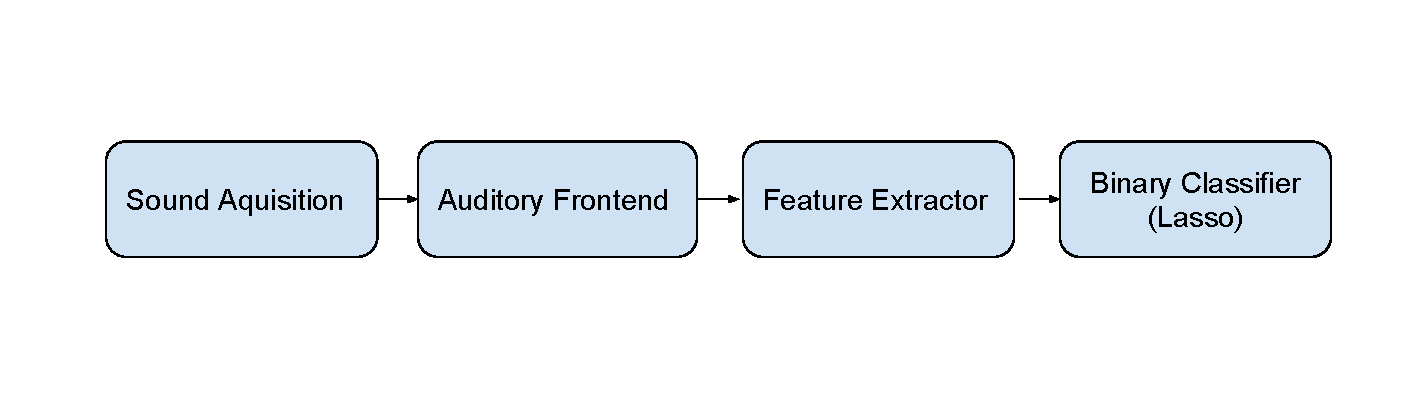
\includegraphics[scale=0.5]{../image/chapter1/identification-pipeline.pdf}
	\caption{Identification Pipeline}
	\label{fig:id-pipeline}
\end{figure}

%TODO: LASSO NOMENCLATURE
In this pipeline, 11 binary one-against-all classifiers using LASSO regression method are trained to accomplish this task. For each of these 11 classes of sound types, a corresponding classifier takes the previously mentioned features $\underline{\mathbf{x}}$ as input and outputs a binary value $y\in \lbrace0,1\rbrace$, where $1$ represents target label. With all of the 11 binary outputs, we can construct a binary vector. An all-zero vector means the sound source is classified as 'anything else' class. This method enables multi-label classification, which means a sound source may be classified as a mix of several classes. 

The accuracy performance of LASSO binary classifier is displayed in Tab.\ref{fig:lassclf}.\footnote{This tabular is extracted from the group talk presentation by Dr. Johannes Mohr on 22.April.2016}%TODO source
Here we use sensitivity, specificity and balanced accuracy to evaluate the classification performance. These three performance metrics are calculated according to the formular below:
\begin{align*}
	sensitivity &= \frac{\#TruePositive}{\#Positive}\\
	specificity &= \frac{\#TrueNegative}{\#Negative}\\
	balanced\quad accuracy &= \frac{sensitivity+specificity}{2}
\end{align*}
As we can see from the bar chart,  Fig.\ref{fig:lassclf}, LASSO classifier performs quite well for class 'female speech', where it achieves $100\%$ sensitivity and $100\%$ specificity. However, the performance of this binary classifier is not so satisfying at class 'engine' with $66\%$ sensitivity and $82\%$ specificity. 

\begin{figure}[h!]
\caption{LASSO Binary Classification Performance}
\label{fig:lassclf}
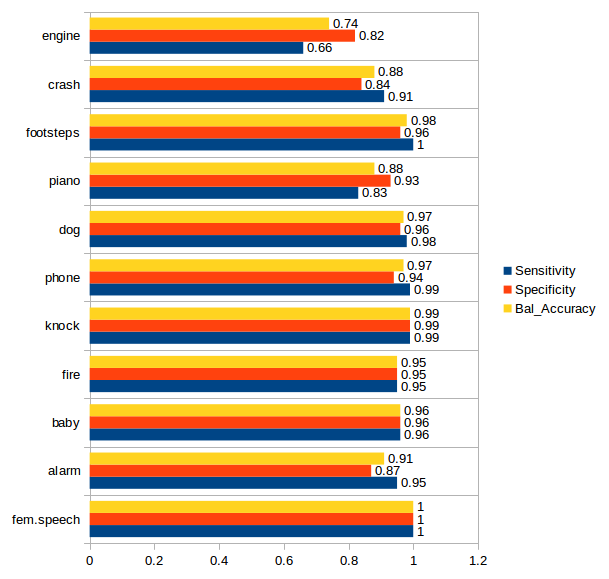
\includegraphics{../image/chapter1/LASSO_results.png}
\end{figure}

\section{Deep Neural Networks}
\label{sec:deepNN}
%motivation(DNN can learn features rather than define them->compare to sec.1.2.2)\\
%related applications,\\
%subsections for DNN(components introduction,caffe)
\subsection{Motivation}
In previous sections, we've seen LASSO binary classifier as a solution to sound type classification problem. In the sound type classification module of the Two!Ears system, handcrafted features(rate maps and AMS features) are taken as the input feature vectors of LASSO binary classifiers. In such simply structured supervised learning model, the quality of features is critical. However, the choice of good features is quite difficult. 

Instead of keeping working hard on feature selection, we now introduce deep neural networks(DNNs) to solve the problem. DNNs can learn features with multiple layers and find high level abstractions in data rather than simply using handcrafted features. Because of such excellent characteristic, DNNs are widely used in a variety of machine learning applications. For example, in automatic speech recognition, DNNs are used to train bottleneck features\cite{zhang2014extracting}. Also in computer vision, DNNs are excellent at learning a good representation of the visual inputs, which can be used to do semantic image segmentation\cite{krizhevsky2012imagenet}. 
\subsection{DNN Structures}
%TODO
A deep neural network (DNN) is an artificial neural network (ANN) with multiple hidden layers of units between the input and output layers\cite{bengio2009learning}\cite{schmidhuber2015deep}. Each layer is made of neurons with learnable weights and biases as parameters of the whole network. Each neuron takes the inner product of outputs from previous layers or input feature vectors with corresponding weights as input and applies an activation function. The common choice of the activation function is the sigmoid function. Fig.\ref{fig:dnnstruc} shows a regular deep neural network structure. If all of the neurons in each layer of the network are fully connected to all activation neurons in the previous layer, such a network is called fully connected neural network.
\begin{figure}
	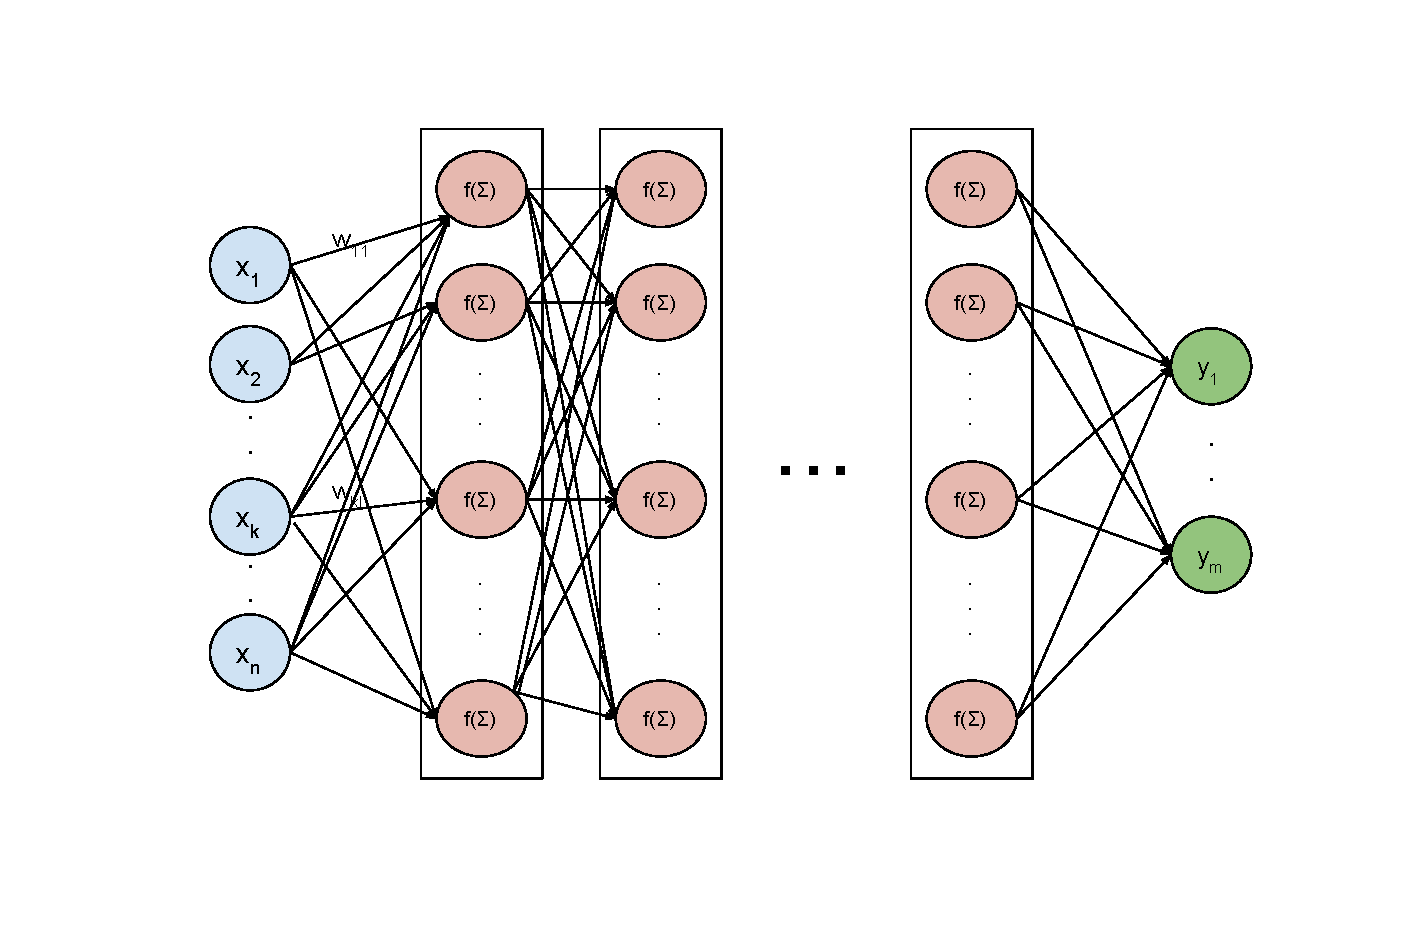
\includegraphics[scale=0.5]{../image/chapter1/dnnstruc.pdf}
	\caption{Deep neural network structure}
	\label{fig:dnnstruc}
\end{figure}

However, such structure is not so efficient with multi-dimensional data like images. Considering a fully connected neural network, the amount of paramters increases with the size of inputs and the number of hidden layers. Too many parameters during training process usually leads to overfitting problem. In this thesis, a variant of regular DNN ,convolutional neural network(CNN), is constructed to solve the problem.

\subsubsection*{Convolutional Neural Networks}
\textit{Convolutional Neural Networks (CNN) are biologically-inspired variants of MLPs(Multilayer Perceptron). }\cite{deeplrn01}

The layers of a CNN have neurons arranged in 3 dimensions: width, height, depth. Instead of following the full connection manner, the neurons of layers in CNNs will be only connected to a small region of layer before it. Such region is called receptive field. In this way, the amount of parameters to be learned is decreased compared with fully connected neural networks. Also parameter sharing scheme is used in Convolutional Layers to control the number of parameters\cite{lecun1995convolutional}. In each layer a new data volume is constructed with corresponding layer parameters. At last, an output volume, which is usually one dimensional vector, is constructed as the final output score.

\subsection{Caffe Toolbox}
Caffe\cite{jia2014caffe} is a deep learning framework. It is developed by the Berkeley Vision and Learning Center (BVLC) and by community contributors. Yangqing Jia created the project during his PhD at UC Berkeley. Caffe is released under the BSD 2-Clause license. In this thesis, I used caffe as the toolbox to implement the convolutional neural networks for sound type classification.

Caffe is written in C++ and it also provides the users with command line, Python, and MATLAB interfaces. The command line interface is the caffe tool for model training, scoring, and diagnostics. All training requires a solver configuration file. In this configuration file, the optimization method and its corresponding parameters are defined. To create a Caffe model you need to define the model architecture in a protocol buffer definition file. In solver configuration file, the full path of the model architecture definition file should also be defined.\footnote{For further details, please refer to the official website of caffe:http://caffe.berkeleyvision.org/}

Caffe provides a variety of layers for users. Generally there are 5 types of layers: vision layers, loss layers, activation/neuron layers, data layers and common layers.
\begin{itemize}
\item  Vision Layers:\\
Convolution, Pooling, Local Response Normalization(LRN),im2col\\
Vision layers  take images as input and produce new images as output. In this thesis, Convolution and Pooling layers were used.
\item Loss Layers:\\
\\Softmax, Sum-of-Squares/Euclidean, Hinge/Margin, Sigmoid Cross-Entropy, Infogain, Accuracy and Top-k\\
Loss layers compare an output to a target and assign cost. During the training stage, the loss itself is computed by the forward pass and the gradient w.r.t. the loss is computed by the backward pass. In this way, loss layer drives the learning process by minimizing the loss. In this thesis, Softmax and Sigmoid Cross-Entropy were used.

\item Activation/Neuron Layers:\\ 
ReLU / Rectified-Linear and Leaky-ReLU, Sigmoid,TanH / Hyperbolic Tangent,Absolute ,Power,BNLL\\
Activation / Neuron layers are element-wise operators, taking one bottom blob and producing one top blob of the same size. In this thesis, ReLU and Sigmoid layers were used.
\item Data Layers:\\
Database, In-Memory, HDF5 Input, HDF5 Output, Images, Windows, Dummy\\
Data enters Caffe through data layers.  Use different types of data layers w.r.t different data sources. In this thesis,HDF5Data layers was used, as the handcrafted features, rate maps and AMS features, were written into hdf5 files.
\item Common Layers:\\
InnerProduct,Splitting,Flattening,Reshape,Concatenation,Slicing, Elementwise Operations,Argmax,Softmax,Mean-Variance Normalization
\\
Common Layers are implemented for simple data operations.
In this thesis, InnerProduct, Concatenation,Slicing and Sigmoid layers were used.
\end{itemize}


\section{Aims of Thesis}
In my thesis, I investigate different architectures of DNNs and different loss functions to improve the  performance of this sound type classification system. I also tried to use data augmentation to overcome the overfitting problem.

%*******************************************************************************
%****************************** Second Chapter *********************************
%*******************************************************************************

\chapter{My second chapter}

\ifpdf
    \graphicspath{{Chapter2/Figs/Raster/}{Chapter2/Figs/PDF/}{Chapter2/Figs/}}
\else
    \graphicspath{{Chapter2/Figs/Vector/}{Chapter2/Figs/}}
\fi


\section[Short title]{Reasonably long section title}

% Uncomment this line, when you have siunitx package loaded.
%The SI Units for dynamic viscosity is \si{\newton\second\per\metre\squared}.
I'm going to randomly include a picture Figure~\ref{fig:minion}.


If you have trouble viewing this document contact Krishna at: \href{mailto:kks32@cam.ac.uk}{kks32@cam.ac.uk} or raise an issue at \url{https://github.com/kks32/phd-thesis-template/}


\begin{figure}[htbp!] 
\centering    

\includegraphics[width=1.0\textwidth]{minion}
\caption[Minion]{This is just a long figure caption for the minion in Despicable Me from Pixar}
\label{fig:minion}
\end{figure}


\section*{Enumeration}
\begin{enumerate}
\item The first topic is dull
\item The second topic is duller
\begin{enumerate}
\item The first subtopic is silly
\item The second subtopic is stupid
\end{enumerate}
\item The third topic is the dullest
\end{enumerate}

\section*{itemize}
\begin{itemize}
\item The first topic is dull
\item The second topic is duller
\begin{itemize}
\item The first subtopic is silly
\item The second subtopic is stupid
\end{itemize}
\item The third topic is the dullest
\end{itemize}

\section*{description}
\begin{description}
\item[The first topic] is dull
\item[The second topic] is duller
\begin{description}
\item[The first subtopic] is silly
\item[The second subtopic] is stupid
\end{description}
\item[The third topic] is the dullest
\end{description}


\clearpage

\tochide\section{Hidden section}
\textbf{Lorem ipsum dolor sit amet}, \textit{consectetur adipiscing elit}. In magna nisi, aliquam id blandit id, congue ac est. Fusce porta consequat leo. Proin feugiat at felis vel consectetur. Ut tempus ipsum sit amet congue posuere. Nulla varius rutrum quam. Donec sed purus luctus, faucibus velit id, ultrices sapien. Cras diam purus, tincidunt eget tristique ut, egestas quis nulla. Curabitur vel iaculis lectus. Nunc nulla urna, ultrices et eleifend in, accumsan ut erat. In ut ante leo. Aenean a lacinia nisl, sit amet ullamcorper dolor. Maecenas blandit, tortor ut scelerisque congue, velit diam volutpat metus, sed vestibulum eros justo ut nulla. Etiam nec ipsum non enim luctus porta in in massa. Cras arcu urna, malesuada ut tellus ut, pellentesque mollis risus.Morbi vel tortor imperdiet arcu auctor mattis sit amet eu nisi. Nulla gravida urna vel nisl egestas varius. Aliquam posuere ante quis malesuada dignissim. Mauris ultrices tristique eros, a dignissim nisl iaculis nec. Praesent dapibus tincidunt mauris nec tempor. Curabitur et consequat nisi. Quisque viverra egestas risus, ut sodales enim blandit at. Mauris quis odio nulla. Cras euismod turpis magna, in facilisis diam congue non. Mauris faucibus nisl a orci dictum, et tempus mi cursus.

Etiam elementum tristique lacus, sit amet eleifend nibh eleifend sed \footnote{My footnote goes blah blah blah! \dots}. Maecenas dapibu augue ut urna malesuada, non tempor nibh mollis. Donec sed sem sollicitudin, convallis velit aliquam, tincidunt diam. In eu venenatis lorem. Aliquam non augue porttitor tellus faucibus porta et nec ante. Proin sodales, libero vitae commodo sodales, dolor nisi cursus magna, non tincidunt ipsum nibh eget purus. Nam rutrum tincidunt arcu, tincidunt vulputate mi sagittis id. Proin et nisi nec orci tincidunt auctor et porta elit. Praesent eu dolor ac magna cursus euismod. Integer non dictum nunc.


\begin{landscape}

\section*{Subplots}
I can cite Wall-E (see Fig.~\ref{fig:WallE}) and Minions in despicable me (Fig.~\ref{fig:Minnion}) or I can cite the whole figure as Fig.~\ref{fig:animations}


\begin{figure}
  \centering
  \begin{subfigure}[b]{0.3\textwidth}
    
\includegraphics[width=\textwidth]{TomandJerry}
    \caption{Tom and Jerry}
    \label{fig:TomJerry}   
  \end{subfigure}             
  \begin{subfigure}[b]{0.3\textwidth}
    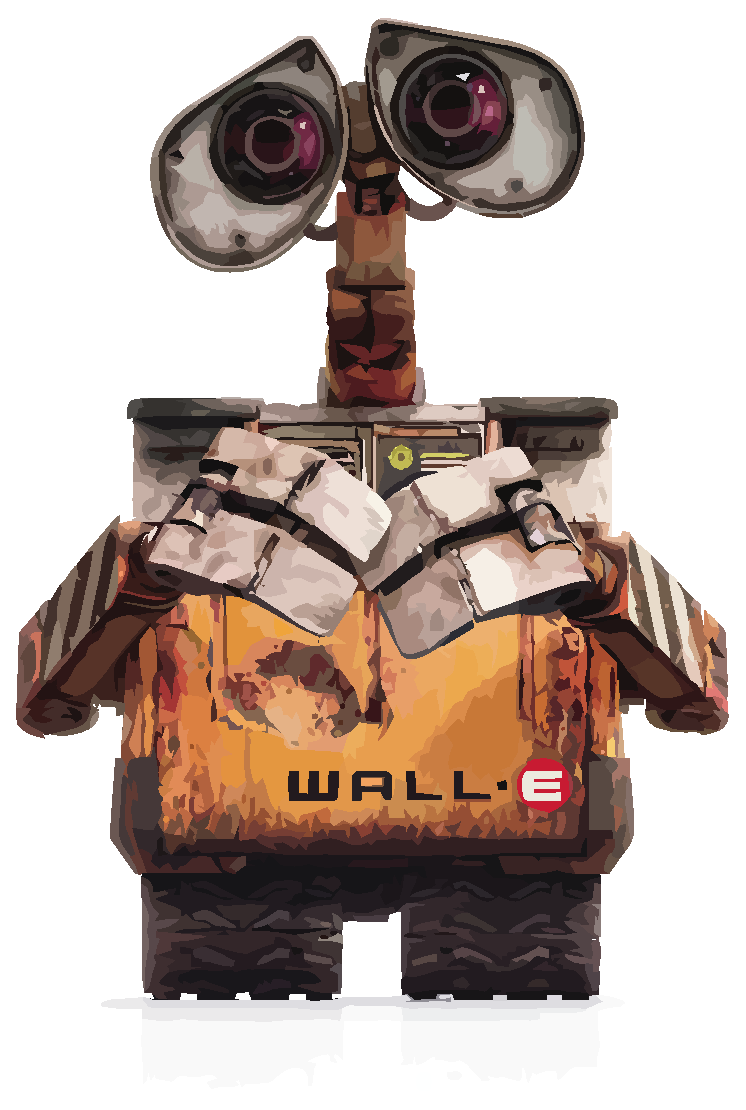
\includegraphics[width=\textwidth]{WallE}
    \caption{Wall-E}
    \label{fig:WallE}
  \end{subfigure}             
  \begin{subfigure}[b]{0.3\textwidth}
    
\includegraphics[width=\textwidth]{minion}
    \caption{Minions}
    \label{fig:Minnion}
  \end{subfigure}
  \caption{Best Animations}
  \label{fig:animations}
\end{figure}


\end{landscape}

\chapter{Data Augmentation}
\label{chap:dataAug}
In this Chapter, data augmentation is introduced to control the overfitting problem. For sound type classification, there are mainly two policies for data augmentation. The effects of different data augmentation policies will also be discussed in this chapter.
\section{Overview and Motivation}
The experiment results in previous chapter show that the training of SigmoidCrossEntropy model meets the overfitting problem. Overfitting usually comes from over trained parameters. If we consider this problem in another way, that is if we have adequate training data to abstract the high level data structure, it may control the overfitting problem to a certain extent. 

Data augmentation was adopted by Krizhevsky et al. to combat the overfitting problem for ImageNet Classification.\cite{krizhevsky2012imagenet} "The easiest and most common method to reduce overfitting on image data is to artificially enlarge the dataset using label-preserving transformations."

What data augmentation does in my experiments is to randomly shift the rate maps and AMS feature over time and frequency domain. Intuitively data augmentation increase the irrelevant variability of training data, which helps the model to find a high level abstraction of the data.  Shifting over time domain only and shifting over both time and frequency domain can be seen as two shifting policies. 

However, such operation is not implemented in Caffe. In the meanwhile, Caffe provides a special type of layer, Python layer, which enables Caffe users to implement self-defined layers in python. I implemented a Python layer for the augmentation operation. The missed data values due to shifting operation are replaced by normal distributed vectors with mean and covariance matrix calculated from the original input features. Instead of padding with constant values, padding with normal distributed vectors add noise in the data rather than changing the data pattern. Such noise adds the classification irrelevant variability in the training data and hence may control the overfitting problem. The shifting step size is randomly generated in each iteration. I also set a range for the shifting steps, this range can be defined by users through the layer parameters. I experimented on a series of this range parameters. 

In the following sections, the parameter settings will be described in form $T(minT,maxT),F(minF,maxF)$. $T$ means shifting over time domain. The shifting step in each forward propagation iteration is a integer, which is uniformly distributed in range $(minT,maxT)$. One shifting step means shifting by one time frame. Positive step means shifting left, while negative step means shifting right. $F$ means shifting over frequency domain. The same as shifting over time domain, the shifting step in each forward propagation iteration over frequency domain is also a integer, which is uniformly distributed in range $(minF,maxF)$. One shifting step over frequency domain means shifting by one frequency channel. Positive step means shifting to higher frequency channels, while negative step means shifting to lower frequency channels. 


\section{Methods}
To compare the performance statistically, I carried out dependent t-tests using the 11-dimensional statistics(performance metrics) between two experiments. T-tests are widely used to determine if two sets of data are significantly different from each other. Large p-value, e.g. greater than 0.05 or 0.1,  rejects the null hypothesis of identical average scores. Small p-value smaller than the threshold, e.g. $0.01$, $0.05$,$0.1$, rejects the null hypothesis of equal averages. In this way, the comparison of performance between two experiments can be seen from this statistic, p-value.
\section{Results and Discussion}
In this section I will mainly compare the experiment results in three steps. Firstly I will compare the new model with data augmentation with the old model in previous chapter. Secondly I will compare 2 shifting policies, shifting over time domain and shifting over both time and frequency domain. At last I will compare different settings of the shifting range parameters used in the Python layer to roughly get a best setting of parameters.
\subsection{Data Augmentation effects}
\label{subsec:dataaug}
In the experiment with data augmentation, I set the shifting range to $T(-30,30)$. The other experiment result to compared with is the SigmoidCrossEntropy model from Chapter \ref{chap:architecture}. 

The experiment results are shown in Fig.\ref{fig:balcompare1}. Two vertical lines represent for the mean value lines for these two experiments. The model with data augmentation outperforms the SigmoidCrossEntropy model for most sound type classes. I also carried out a dependent t-test with the balanced accuracy statistics from these two experiments, the p-value I got is $0.049577<0.05$ which means the performance statistics of two models are indeed significantly different from each other. Data augmentation improved the model performance.
\begin{figure}[h!]
	\caption{Balanced accuracy of two models, shift over T(-30,30)}
	\label{fig:balcompare1}
	\centering
	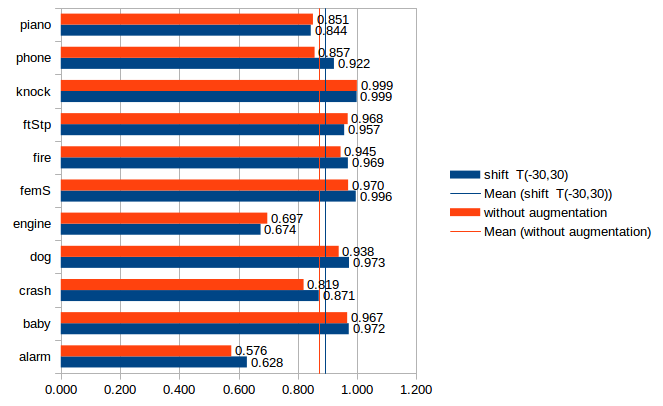
\includegraphics[scale=0.85]{../image/chapter3/bal_acc_T1.png}
\end{figure}

\subsection{Shifting policies}
Besides shifting over time domain, shifting over both frequency domain and time domain is another shifting policy. Shifting over time domain adds the variability of recording delay. Shifting over frequency domain adds the variability of basic frequency of the sound source. These two variability can be both considered as irrelevant.
\begin{figure}[h!]
	\caption{Balanced accuracy of two shifting policies,shift over  T(-30,30),shift over T(-30,30),F(-8,8)}
	\label{fig:balcompare2}
	\centering
	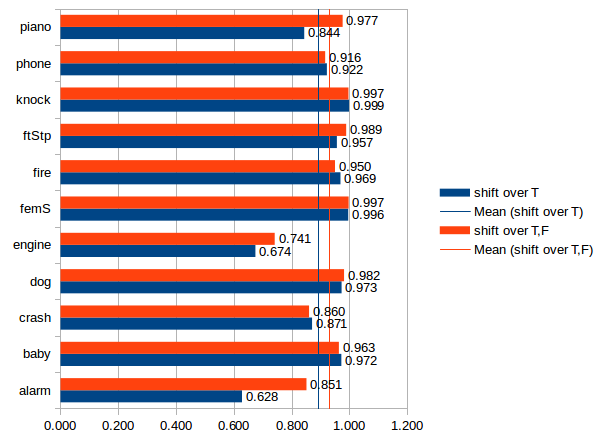
\includegraphics[scale=0.9]{../image/chapter3/bal_acc_TvsF.png}
\end{figure}
The parameter setting for shifting over time domain policy is the same as that described in section \ref{subsec:dataaug}, which is $T(-30,30)$. The parameter setting for shifting over time and frequency domain is $T(-30,30),F(-8,8)$.
 For 6 of the sound types, shifting over time and frequency domain outperforms shifting over time domain. The averaged balanced accuracy over 11 sound types of shifting over time and frequency domain is greater than the other shifting policy. So in the following experiments of shifting parameters, I preferred to adopt the shifting over time and frequency policy.
 
\subsection{Shifting Parameters}
To roughly find a good parameter settings for data augmentation, I carried out three experiments with different parameter settings:
\begin{itemize}
	\item $T(-30,30),F(-8,8)$
	\item $T(-15,15),F(-4,4)$
	\item $T(-40,40),F(-8,8)$
\end{itemize}

 Fig.\ref{fig:balcompare3} shows the balanced accuracy and Fig.\ref{fig:senscompare} shows the sensitivity metric of these three experiments. 
% which means shift steps over time domain in range (-15,15) and shift steps over frequency domain in range (-4,4). 
\begin{figure}[h!]
	\caption{Balanced accuracy of 3 parameter settings}
	\label{fig:balcompare3}
	\centering
	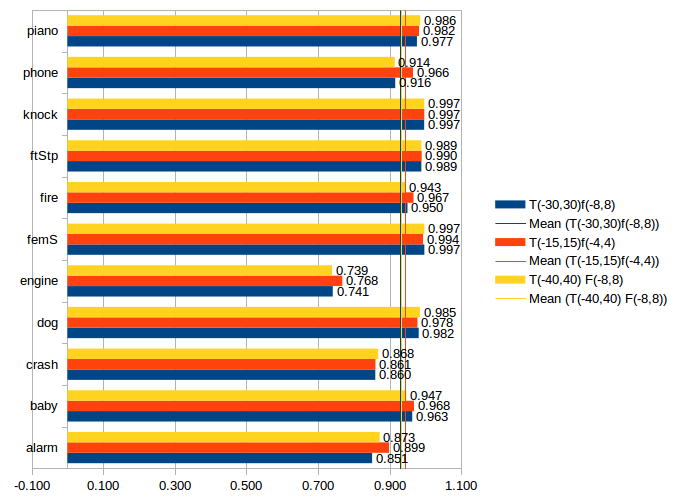
\includegraphics[scale=0.85]{../image/chapter3/bal_params.png}
\end{figure}
\begin{figure}[h!]
	\caption{Sensitivity of 3 parameter settings}
	\label{fig:senscompare}
	\centering
	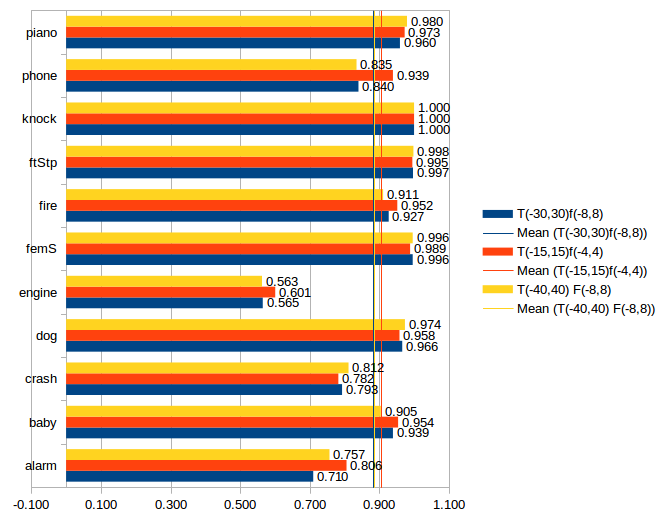
\includegraphics[scale=0.85]{../image/chapter3/sens_params.png}
\end{figure}
From the vertical lines in the diagram, which indicates the mean performance metrics over sound type classes, we can see that the averaged balanced accuracy and the averaged sensitivity of parameter setting $T(-15,15),F(-4,4)$ are the highest among all of these three parameter settings. So currently the  advisable shifting parameters would be $T(-15,15)F(-4,4)$.

\subsection{Summarize and Conclusion}
\label{subsec:sftparams}
The averaged balanced accuracy over 11 sound type classes of the experiments in this chapter are listed in Tab.\ref{tab:balfullresults}. The performance metric values in bold are the best values among these 5 experiments. The best balanced accuracy is acquired in the experiment with data augmentation with parameter setting $T(-15,15)F(-4,4)$.
\begin{table}
\begin{tabular}{|c|c|c|c|}
	\hline		&	\textbf{balanced accuracy}	&	\textbf{sensitivity}	&	\textbf{specificity	}\\
	\hline	\textbf{no data augmentation}	&	0.872	&	0.752	&	\textbf{0.991}	\\
	\hline	\textbf{T(-30,30)}	&	0.891	&	0.799	&	0.984	\\
	\hline	\textbf{T(-30,30),F(-8,8)}	&	0.929	&	0.881	&	0.978	\\
	\hline	\textbf{T(-15,15)F(-4,4)}	&	\textbf{0.943}	&	\textbf{0.905}	&	0.981	\\
	\hline	\textbf{T(-40,40)F(-4,4)}	&	0.931	&	0.885	&	0.977	\\
	\hline 
\end{tabular} 
\label{tab:balfullresults}
\caption{Averaged performance metrics for 5 experiments}
\end{table}
Also if we compare the ROC curves of SigmoidCrossEntropy model from previous chapter and the model with data augmentation constructed in this chapter, we can see that the 'auc'(area under curve) values of SigmoidCrossEntropy model with data augmentation for all of these 11 sound type classes are over $0.95$, while the 'auc' values of SigmoidCrossEntropy model without data augmentation for sound type 'alarm' and 'engine' are below $0.95$.  Thus we can conclude that data augmentation can be adopted as a method to control overfitting problem. The ROC curves are shown in Fig.\ref{fig:rocAug}
\begin{figure}[t!]
	\centering
	\subfigure[SigmoidCrossEntropy model without data augmentation]{
		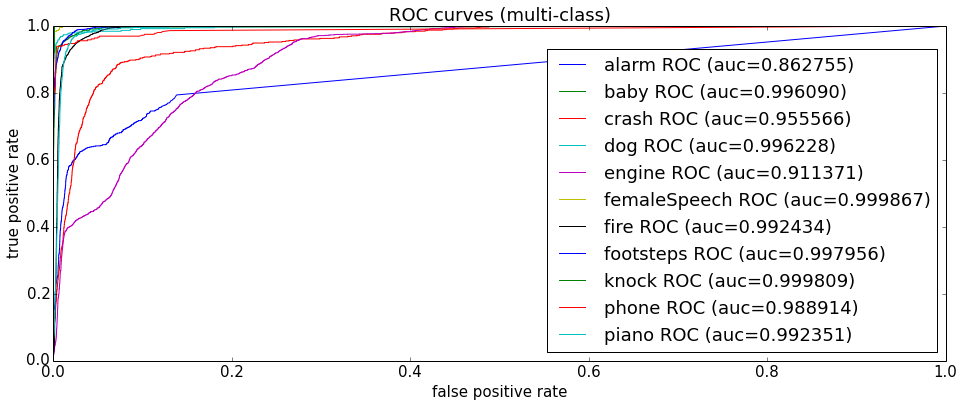
\includegraphics[scale =0.4] {../image/chapter3/rocSCE.png}
		\label{fig:subfig1}
	}
	\subfigure[SigmoidCrossEntropy model with data augmentation $T(-15,15),F(-4,4)$]{
		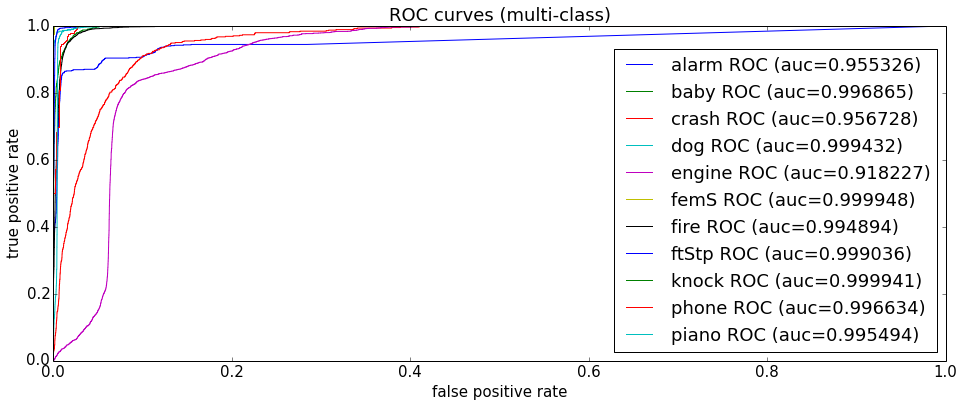
\includegraphics[scale =0.4] {../image/chapter3/rocT15F4.png}
		\label{fig:subfig2}
	}
	\caption{ROC Curves for models with and without Data Augmentation}
	\label{fig:rocAug}
\end{figure}
%\chapter{Comparison of Optimization Algorithms}
%Discuss about different solver types(SGD,Adam,Adadelta,) related works
%"SGD"(Stochastic Gradient Descent)\\
%"AdaGrad"(Adaptive Gradient)\\
%"Adam"(Adaptive Moment Estimation)\\
%"AdaDelta"\\
%"NAG"(Nesterov’s accelerated gradient)\\
%"RMSprop"\\
\label{chap:solver}
In Caffe toolbox, optimization algorithms corresponds to the solver types. There are 6 types of solver implemented in Caffe:
\begin{itemize}
	\item Stochastic Gradient Descent (type: "SGD"),
\item	AdaDelta (type: "AdaDelta"),
\item	Adaptive Gradient (type: "AdaGrad"),
\item	Adam (type: "Adam"),
\item	Nesterov’s Accelerated Gradient (type: "Nesterov") and
\item	RMSprop (type: "RMSProp")
\end{itemize}
All the experiments carried out in previous sections used Stochastic Gradient Descent as the optimization algorithm.
 
\section{Implementation Details}

\section{Results and Discussion}

%\chapter{Conclusions and Outlook}
\label{chap:conclusion}
%summarize the main findings and draw conclusions\\
%(drp seems doesn't perform good...)\\
%point out future research directions,limitations,
%(maybe more drp layers after layers...\\
%methods to 
%conquer overfitting, more hidden layers,drp,...)
In this thesis, I first constructed three DNN architectures and focused on SigmoidCrossEntropy due to its advantage in extension of multi-label classification and its good receiver operating characteristic as shown in Fig.\ref{fig:rocAug} in section \ref{subsec:sftparams}. The application of data augmentation improves the averaged balanced accuracy by $7.1\%$(from $87.2\%$ to $94.3\%$). In conclusion, data augmentation helps in controlling overfitting problem.

As shown in Chapter\ref{chap:dataAug}, the experiment results are sensitive to parameter settings. In future work, finding a optimal parameters setting could be one research direction. 

Besides data augmentation, there are more options to conquer the overfitting problem, such as adding more dropout layers into the network, altering the kernel size for convolutional layers to decrease the amount of weights in the network. Also good parameters tuning would help a lot when optimizing the DNN architecture. However such optimization is computationally very costly. A full learning process of a DNN model goes through the entire data set multiple times. Each alteration of a hyper parameter requires such a lengthy learning process.
%\include{Chapter6/chapter6}
%\include{Chapter7/chapter7}



% ********************************** Back Matter *******************************
% Backmatter should be commented out, if you are using appendices after References
%\backmatter

% ********************************** Bibliography ******************************
\begin{spacing}{0.9}

% To use the conventional natbib style referencing
% Bibliography style previews: http://nodonn.tipido.net/bibstyle.php
% Reference styles: http://sites.stat.psu.edu/~surajit/present/bib.htm

\bibliographystyle{apalike}
%\bibliographystyle{unsrt} % Use for unsorted references  
%\bibliographystyle{plainnat} % use this to have URLs listed in References
\cleardoublepage
\bibliography{References/references} % Path to your References.bib file


% If you would like to use BibLaTeX for your references, pass `custombib' as
% an option in the document class. The location of 'reference.bib' should be
% specified in the preamble.tex file in the custombib section.
% Comment out the lines related to natbib above and uncomment the following line.

%\printbibliography[heading=bibintoc, title={References}]


\end{spacing}

% ********************************** Appendices ********************************

\begin{appendices} % Using appendices environment for more functunality

% ******************************* Thesis Appendix A ****************************
\chapter{How to install \LaTeX} 

\section*{Windows OS}

\subsection*{TeXLive package - full version}
\begin{enumerate}
\item	Download the TeXLive ISO (2.2GB) from\\
\href{https://www.tug.org/texlive/}{https://www.tug.org/texlive/}
\item	Download WinCDEmu (if you don't have a virtual drive) from \\
\href{http://wincdemu.sysprogs.org/download/}
{http://wincdemu.sysprogs.org/download/}
\item	To install Windows CD Emulator follow the instructions at\\
\href{http://wincdemu.sysprogs.org/tutorials/install/}
{http://wincdemu.sysprogs.org/tutorials/install/}
\item	Right click the iso and mount it using the WinCDEmu as shown in \\
\href{http://wincdemu.sysprogs.org/tutorials/mount/}{
http://wincdemu.sysprogs.org/tutorials/mount/}
\item	Open your virtual drive and run setup.pl
\end{enumerate}

or

\subsection*{Basic MikTeX - \TeX~ distribution}
\begin{enumerate}
\item	Download Basic-MiK\TeX (32bit or 64bit) from\\
\href{http://miktex.org/download}{http://miktex.org/download}
\item	Run the installer 
\item	To add a new package go to Start >> All Programs >> MikTex >> Maintenance (Admin) and choose Package Manager
\item	Select or search for packages to install
\end{enumerate}

\subsection*{TexStudio - \TeX~ editor}
\begin{enumerate}
\item	Download TexStudio from\\
\href{http://texstudio.sourceforge.net/\#downloads}
{http://texstudio.sourceforge.net/\#downloads} 
\item	Run the installer
\end{enumerate}

\section*{Mac OS X}
\subsection*{MacTeX - \TeX~ distribution}
\begin{enumerate}
\item	Download the file from\\
\href{https://www.tug.org/mactex/}{https://www.tug.org/mactex/}
\item	Extract and double click to run the installer. It does the entire configuration, sit back and relax.
\end{enumerate}

\subsection*{TexStudio - \TeX~ editor}
\begin{enumerate}
\item	Download TexStudio from\\
\href{http://texstudio.sourceforge.net/\#downloads}
{http://texstudio.sourceforge.net/\#downloads} 
\item	Extract and Start
\end{enumerate}


\section*{Unix/Linux}
\subsection*{TeXLive - \TeX~ distribution}
\subsubsection*{Getting the distribution:}
\begin{enumerate}
\item	TexLive can be downloaded from\\
\href{http://www.tug.org/texlive/acquire-netinstall.html}
{http://www.tug.org/texlive/acquire-netinstall.html}.
\item	TexLive is provided by most operating system you can use (rpm,apt-get or yum) to get TexLive distributions
\end{enumerate}

\subsubsection*{Installation}
\begin{enumerate}
\item	Mount the ISO file in the mnt directory
\begin{verbatim}
mount -t iso9660 -o ro,loop,noauto /your/texlive####.iso /mnt
\end{verbatim}

\item	Install wget on your OS (use rpm, apt-get or yum install)
\item	Run the installer script install-tl.
\begin{verbatim}
	cd /your/download/directory
	./install-tl
\end{verbatim}
\item	Enter command `i' for installation

\item	Post-Installation configuration:\\
\href{http://www.tug.org/texlive/doc/texlive-en/texlive-en.html\#x1-320003.4.1}
{http://www.tug.org/texlive/doc/texlive-en/texlive-en.html\#x1-320003.4.1} 
\item	Set the path for the directory of TexLive binaries in your .bashrc file
\end{enumerate}

\subsubsection*{For 32bit OS}
For Bourne-compatible shells such as bash, and using Intel x86 GNU/Linux and a default directory setup as an example, the file to edit might be \begin{verbatim}
edit $~/.bashrc file and add following lines
PATH=/usr/local/texlive/2011/bin/i386-linux:$PATH; 
export PATH 
MANPATH=/usr/local/texlive/2011/texmf/doc/man:$MANPATH;
export MANPATH 
INFOPATH=/usr/local/texlive/2011/texmf/doc/info:$INFOPATH;
export INFOPATH
\end{verbatim}
\subsubsection*{For 64bit OS}
\begin{verbatim}
edit $~/.bashrc file and add following lines
PATH=/usr/local/texlive/2011/bin/x86_64-linux:$PATH;
export PATH 
MANPATH=/usr/local/texlive/2011/texmf/doc/man:$MANPATH;
export MANPATH 
INFOPATH=/usr/local/texlive/2011/texmf/doc/info:$INFOPATH;
export INFOPATH

\end{verbatim}



%\subsection{Installing directly using Linux packages} 
\subsubsection*{Fedora/RedHat/CentOS:}
\begin{verbatim} 
sudo yum install texlive 
sudo yum install psutils 
\end{verbatim}


\subsubsection*{SUSE:}
\begin{verbatim}
sudo zypper install texlive
\end{verbatim}


\subsubsection*{Debian/Ubuntu:}
\begin{verbatim} 
sudo apt-get install texlive texlive-latex-extra 
sudo apt-get install psutils
\end{verbatim}

% ******************************* Thesis Appendix B ********************************

\chapter{Installing the CUED class file}

\LaTeX.cls files can be accessed system-wide when they are placed in the
<texmf>/tex/latex directory, where <texmf> is the root directory of the user’s \TeX installation. On systems that have a local texmf tree (<texmflocal>), which
may be named ``texmf-local'' or ``localtexmf'', it may be advisable to install packages in <texmflocal>, rather than <texmf> as the contents of the former, unlike that of the latter, are preserved after the \LaTeX system is reinstalled and/or upgraded.

It is recommended that the user create a subdirectory <texmf>/tex/latex/CUED for all CUED related \LaTeX class and package files. On some \LaTeX systems, the directory look-up tables will need to be refreshed after making additions or deletions to the system files. For \TeX Live systems this is accomplished via executing ``texhash'' as root. MIK\TeX users can run ``initexmf -u'' to accomplish the same thing.

Users not willing or able to install the files system-wide can install them in their personal directories, but will then have to provide the path (full or relative) in addition to the filename when referring to them in \LaTeX.

\end{appendices}

% *************************************** Index ********************************
\printthesisindex % If index is present

\end{document}